\documentclass{acm_proc_article-sp}          % LaTeX 2e 
%\usepackage{latex8}                              % LaTeX 2e 
\usepackage{times}                               % LaTeX 2e 
\usepackage{cite}
\usepackage{graphicx}
%\usepackage{amssymb,amsmath,amsthm}
\usepackage{algorithm,algorithmic}
%\usepackage{wasysym}
\usepackage{url}
\usepackage{subfigure}

\newcommand{\domain}[1]{\mathbb{#1}}
\renewcommand{\algorithmiccomment}[1]{ /* #1 */}
\newtheorem{theorem}{Theorem}

%------------------------------------------------------------------------- 
% take the % away on next line to produce the final camera-ready version 
%\pagestyle{empty}

%------------------------------------------------------------------------- 
\begin{document}

\title{Random Rectilinear Polygon Generation and Dynamic Priority
  Search Tree}

\author{First Author\\
Institution\\
First line of institution address\\ Second line of institution address\\ 
FirstAuthor@institution.com\\
% For a paper whose authors are all at the same institution, 
% omit the following lines up until the closing ``}''.
% Additional authors and addresses can be added with ``\and'', 
% just like the second author.
\and
Second Author\\
Institution2\\
First line of institution2 address\\ Second line of institution2 address\\ 
SecondAuthor@institution2.com\\
}

\maketitle
\thispagestyle{empty}

\begin{abstract}
Two fundamental CAD algorithms for physical design are discussed,
namely random polygon generation and dynamical priority search. 
\end{abstract}

%------------------------------------------------------------------------- 

\section{Introduction}
\label{sec:intro}
Sometimes, even serious research works could make mistakes. 
I describe a story in the following. 
An algorithm for construction of variable
length code with limited maximum word length was first published on an
IEEE transaction in 1984~\cite{vl-code-84}. 
The algorithm basically contains only six steps. 
In 1986, the authors of~\cite{vl-code-86} pointed out that the
algorithm does not always lead to an optimal code and made their
corrections thereafter~\cite{vl-code-86}. 
Unfortunately, the algorithm with their corrections still has
problems. The issue has not been discovered until Hu
tested the algorithm carefully in 1988~\cite{vl-code-88}.

%Testing algorithms
%Daily Unit Testing
%Improve robustness of algorithms
%Test-Driven Development (TDD)
%Speedup the development process 
%Initial solution of an iterative method.
%Gather statistical information - may require random objects have
%desired distribution, such as uniform distribution. 

We once implemented a polygon-cutting algorithm.
We tested it by layout polygons.
Everything looked OK, but in fact there was a bug in our
implementation: it does not handle correctly some special cases. 
The bug was not caught until random polygon was applied. 

Beside testing, random objects can also be used in algorithms. 
For example, the simulated annealing technique for floorplanning
algorithms. Instead of starting with an initial floorplanning that is
all vertical strips, which is obviously not a good solution, one may
start with a random floorplan as shown in Figure~\ref{fig:sf50}.

\begin{figure}[ht]
  \centering
  \scalebox{0.35}{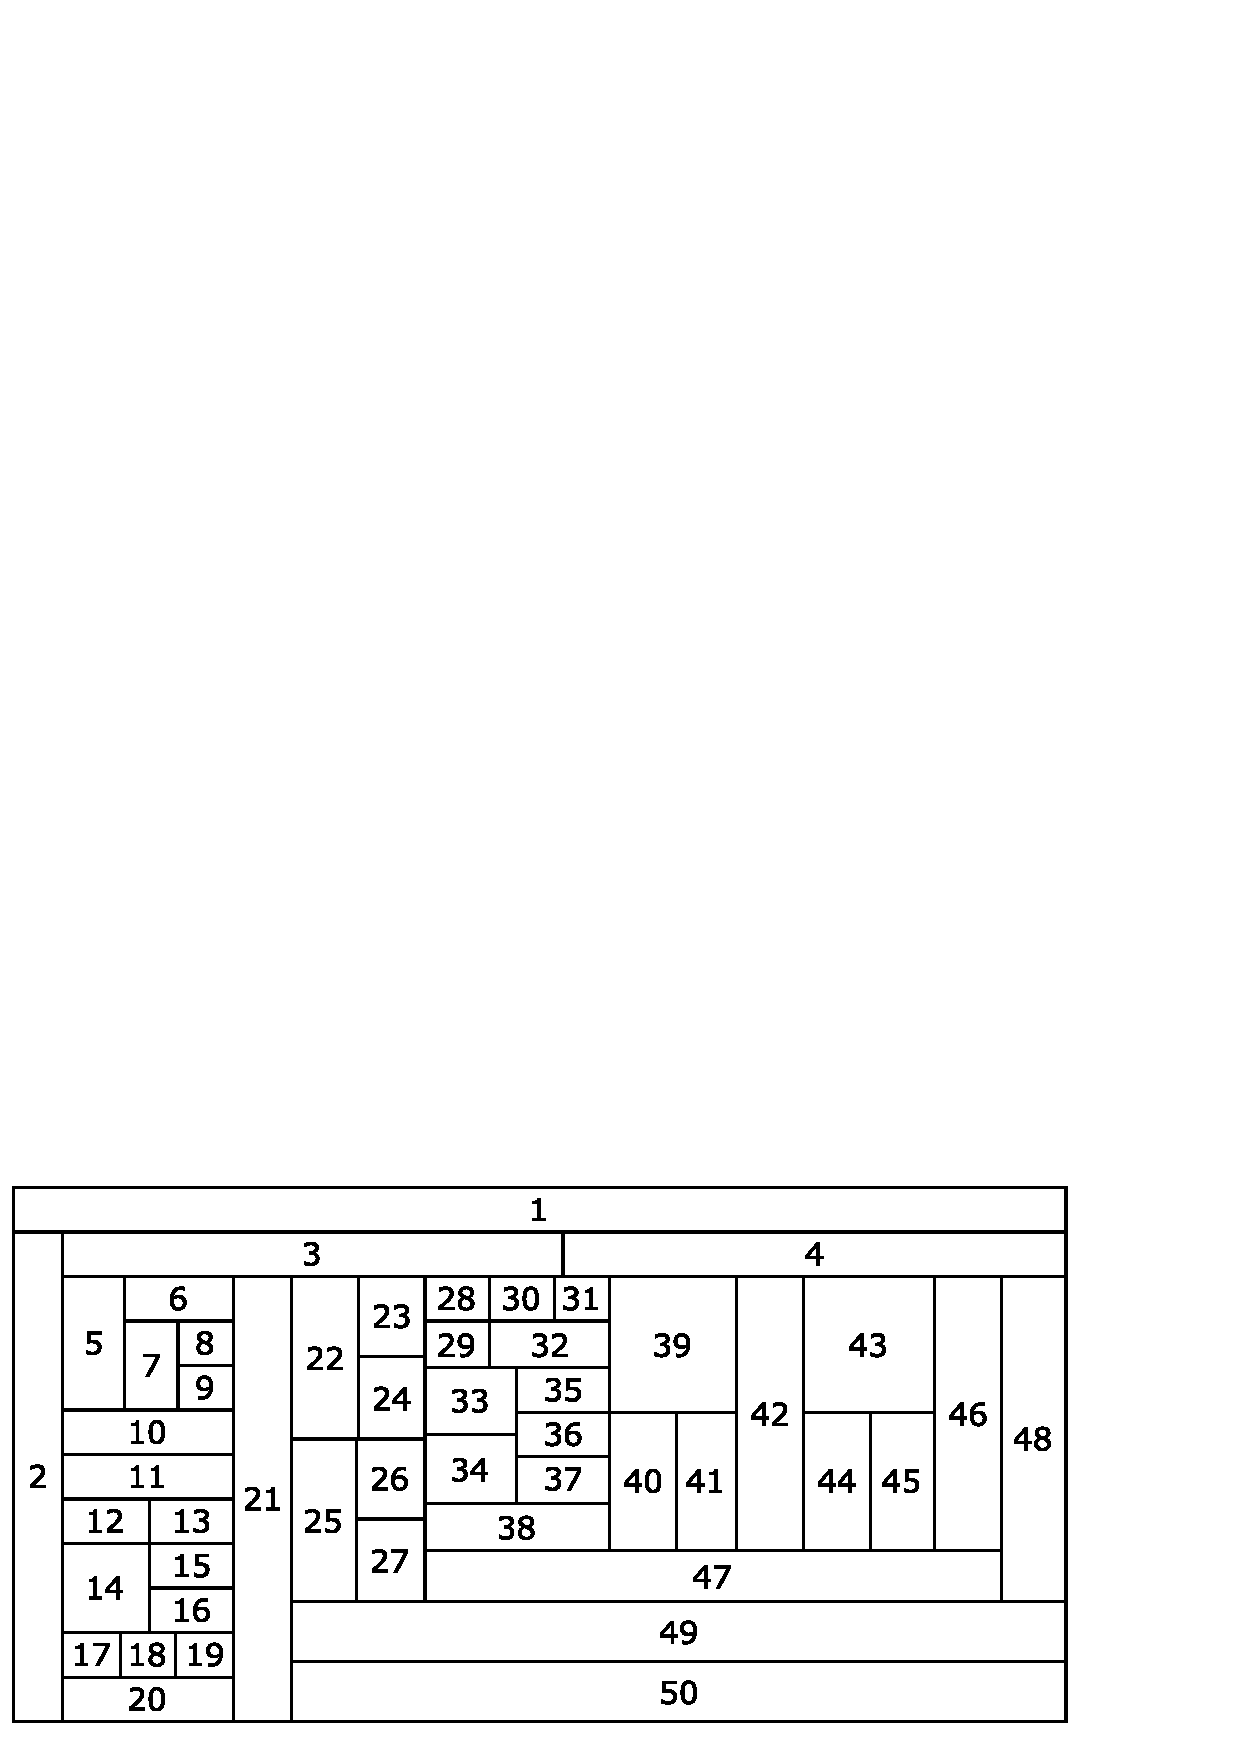
\includegraphics[width=1.0\textwidth]{sf50}}\\
  \caption{Random slicing floorplan with 50 rooms.}\label{fig:sf50}
\end{figure}

Unlike other 2-D data structures such as kd-tree, quad-tree and
R-tree, priority search tree (PST) has not been well noticed in EDA
community. One of the reasons may be that PST is only specialized in a
particular kind of range query, making it unsuitable for general
applications. Another reason is that the implementation of PST is not
trivial, especially one that requires dynamic balancing. Recently, the
speaker has implemented an efficient dynamic PST algorithm in C++. The
query time is less than one second for 10,000 data points. In this
talk, we will present the implementation detail of the algorithm. 

\section{Random Polygon Generation}
\label{sec:rpolygon}
Given a set of 2-dimensional points $P = (p_1, p_2, \cdots, p_n)$. 
A polygon is called \emph{simple} if all segments are
non-intersecting. 
We ask for a random \emph{simple} polygon whose vertices are $P$.

We first review an algorithm for general
\subsection{Random Simple 2-d Polygon}
2-opt move: replace two intersecting edges with two non-intersecting
edges so as to keep the polygon connected.

\begin{algorithm}[ht]
\caption{Random simple polygon}
\label{alg:ellipsoid}
    \begin{algorithmic}[1]
     \REQUIRE a set of $n$ points
      \WHILE{there exists intersection}
        \STATE Perform a 2-opt move.
      \ENDWHILE
    \end{algorithmic}
\end{algorithm}

Note that the algorithm will eventually converge to a simple polygon
because the 2-opt move decreases total length~\cite{zssm-grpgv-96}.
Figure~\ref{fig:polygon} shows the result of random polygon with 500
vertices.

\begin{figure}[ht]
  \centering
  \scalebox{0.35}{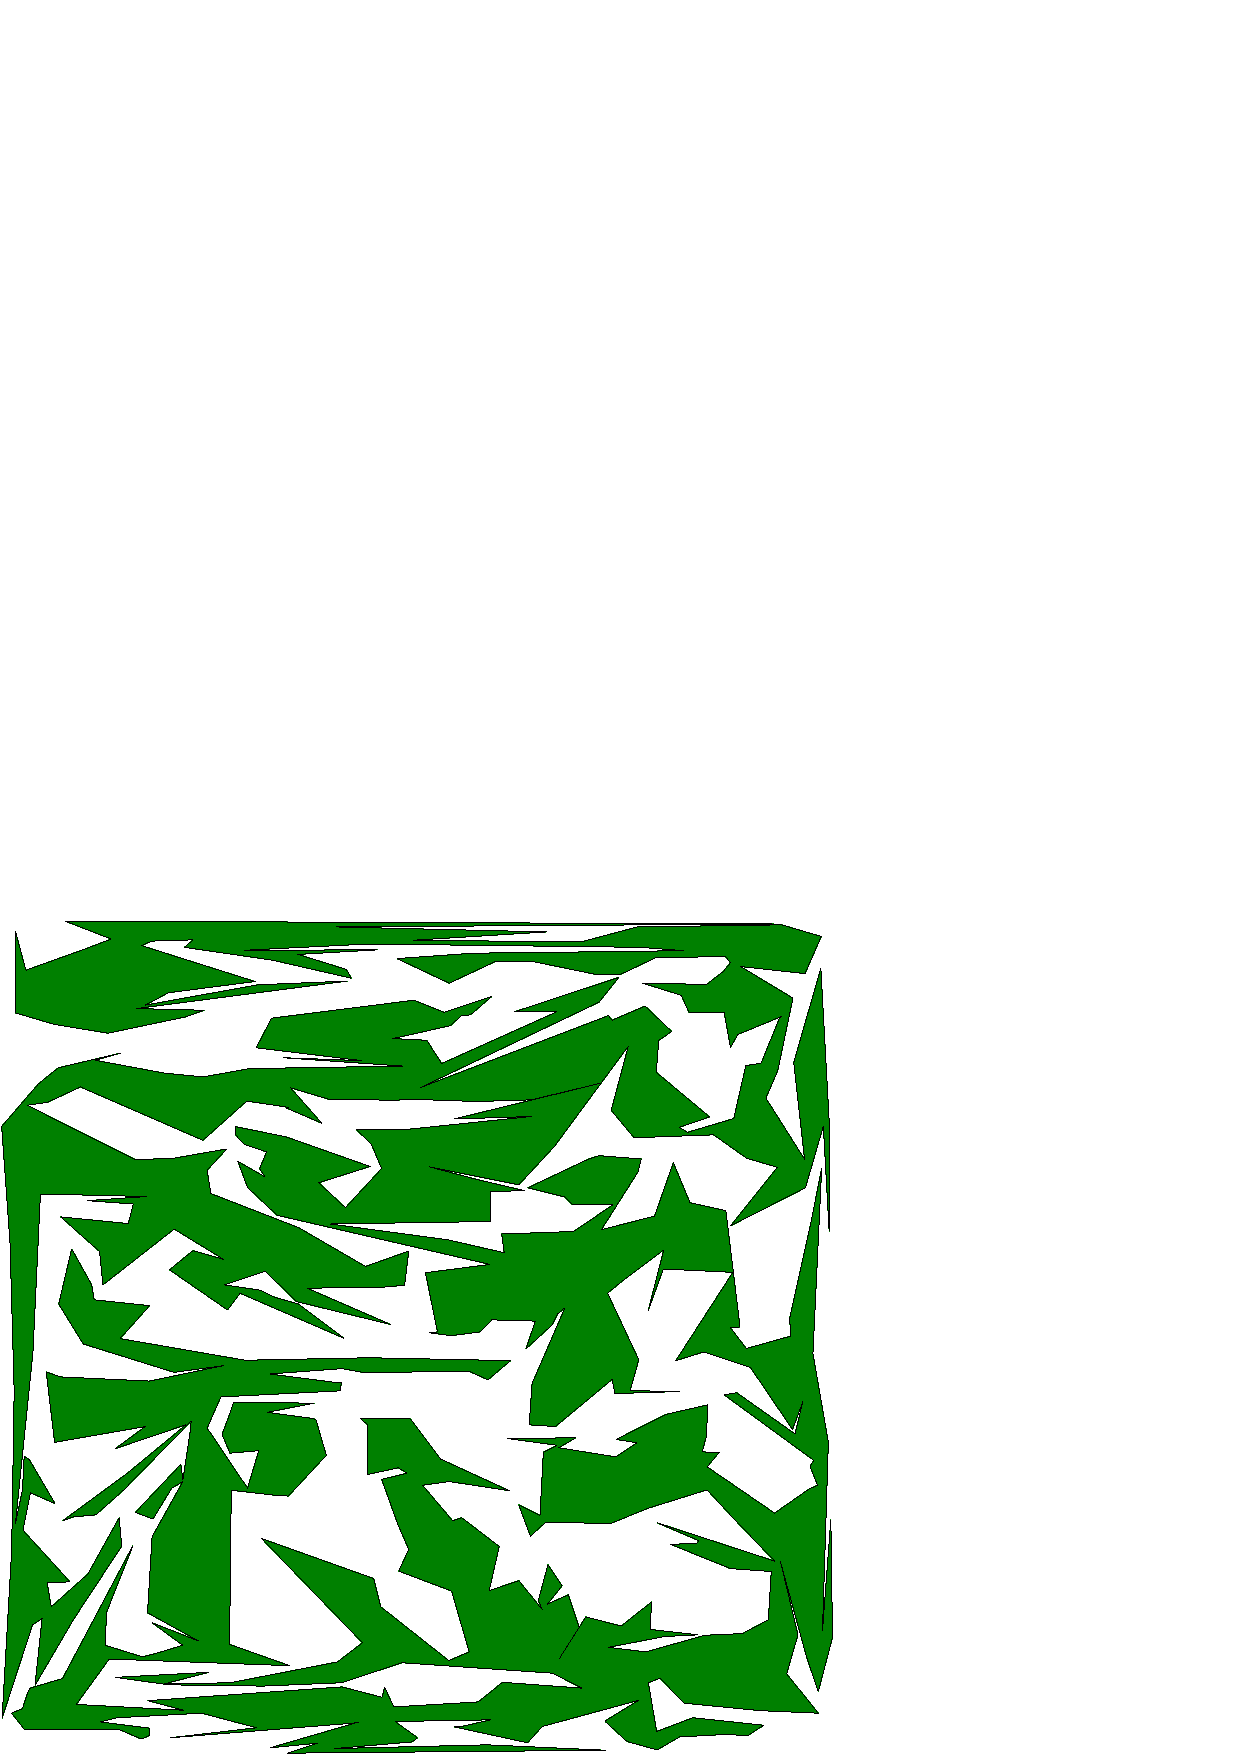
\includegraphics[width=1.0\textwidth]{polygon}}\\
  \caption{Random polygon with 500 vertices.}\label{fig:polygon}
\end{figure}

Theoretical upper bound of the number of 2-opt moves is $O(N^3)$. But
the bound is not tight. Empirically, usually only need $O(N)$. 
The algorithm does not generate simple polygons uniformly.
In fact, it is an open problem if they can be generated uniformly in
polynomial time.


\subsection{Random Rectilinear Polygon}
A polygon is call \emph{rectilinear} polygon if each
segment is either horizontal or vertical. Obviously a rectilinear
polygon can be possible only when $n$ is an even number.

Similar idea to the 2-opt move method:
Note that number of vertices is unchanged.
Special cases: Both two intersecting lines are horizontal (or
vertical) and are in the same direction:


%\begin{figure}[ht]
%  \centering
%  \scalebox{0.35}{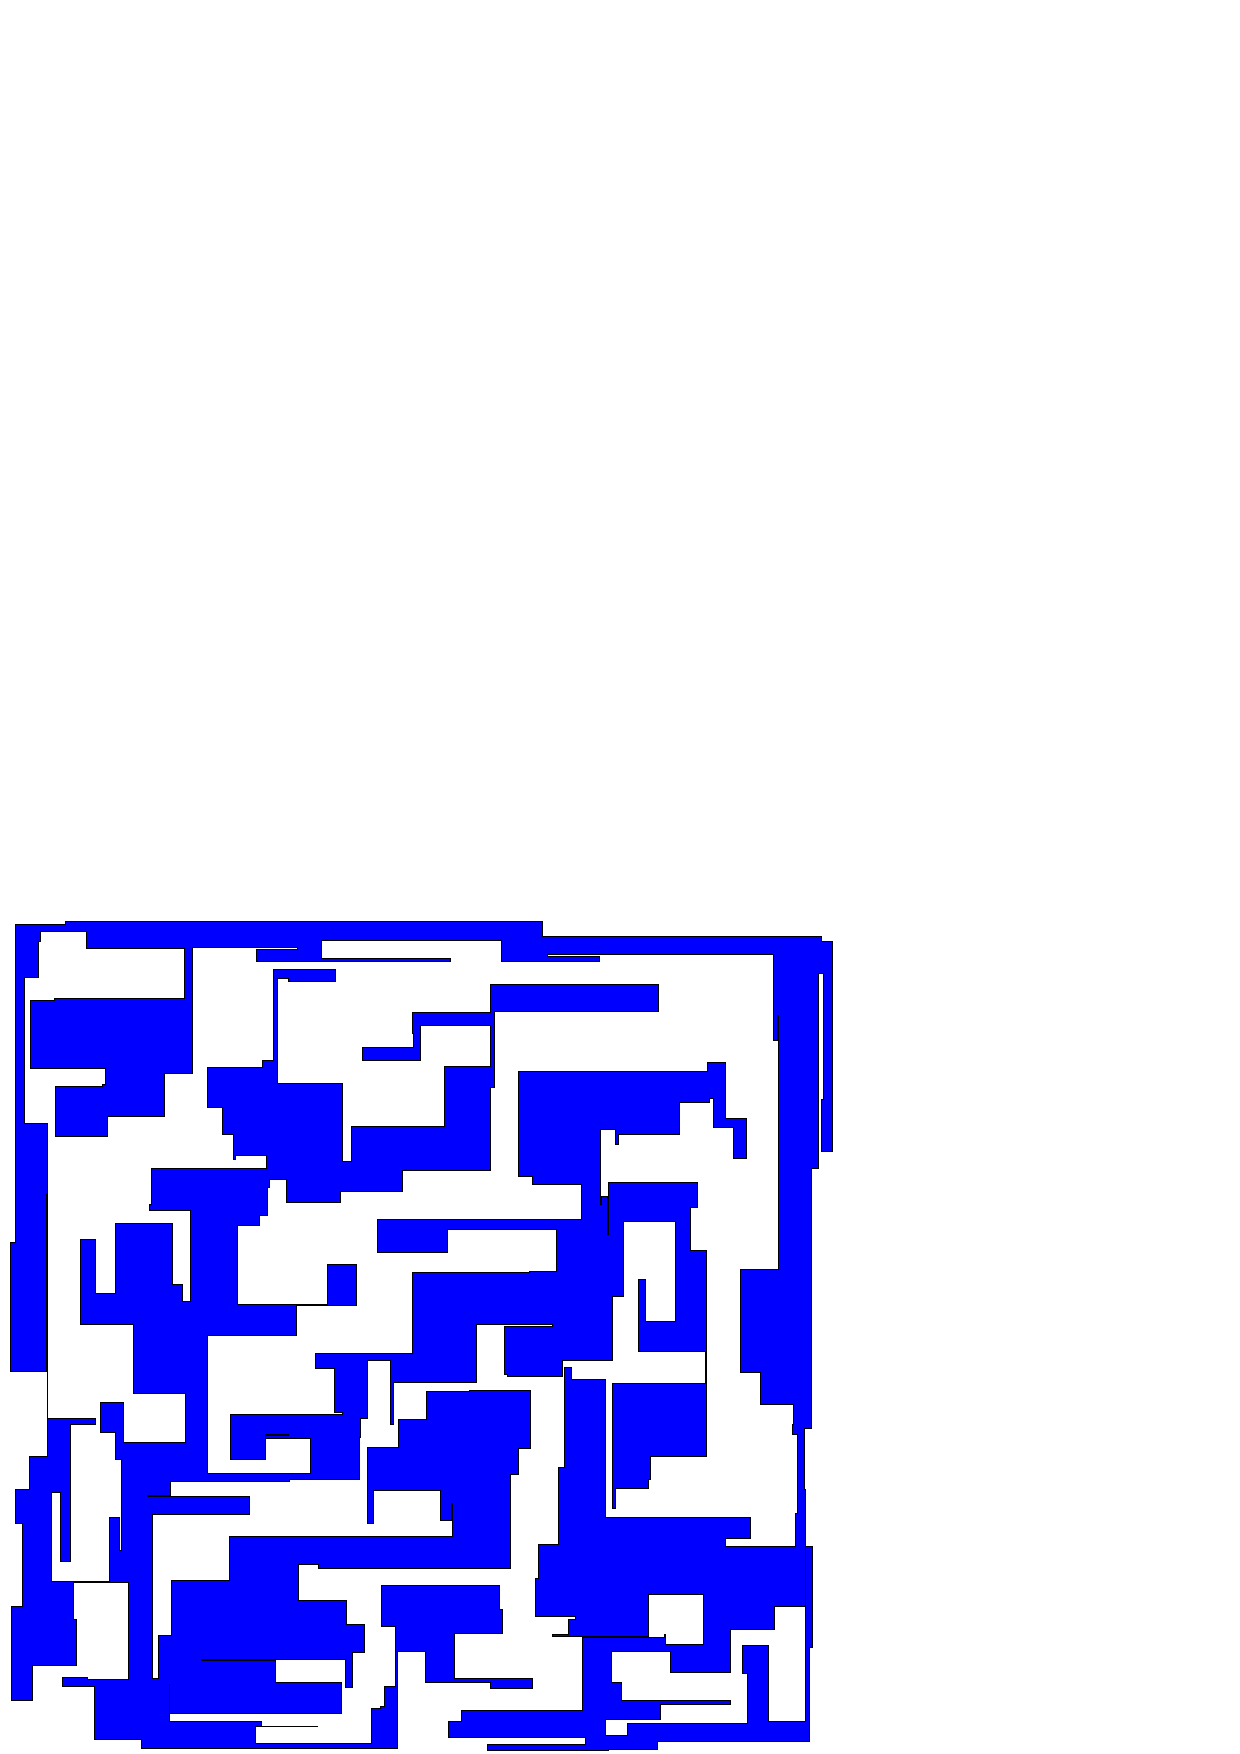
\includegraphics[width=1.0\textwidth]{rpolygon}}\\
%  \caption{Random rectilinear with 500 vertices.}\label{fig:rpolygon}
%\end{figure}

\begin{theorem}
The algorithm eventually converges to a simple rectilinear polygon.
\end{theorem}
\begin{proof}
\end{proof}

Figure~\ref{fig:polygon_cutting} shows an application of testing
polygon cutting algorithm.

\begin{figure}[ht]
  \centering
  \scalebox{0.35}{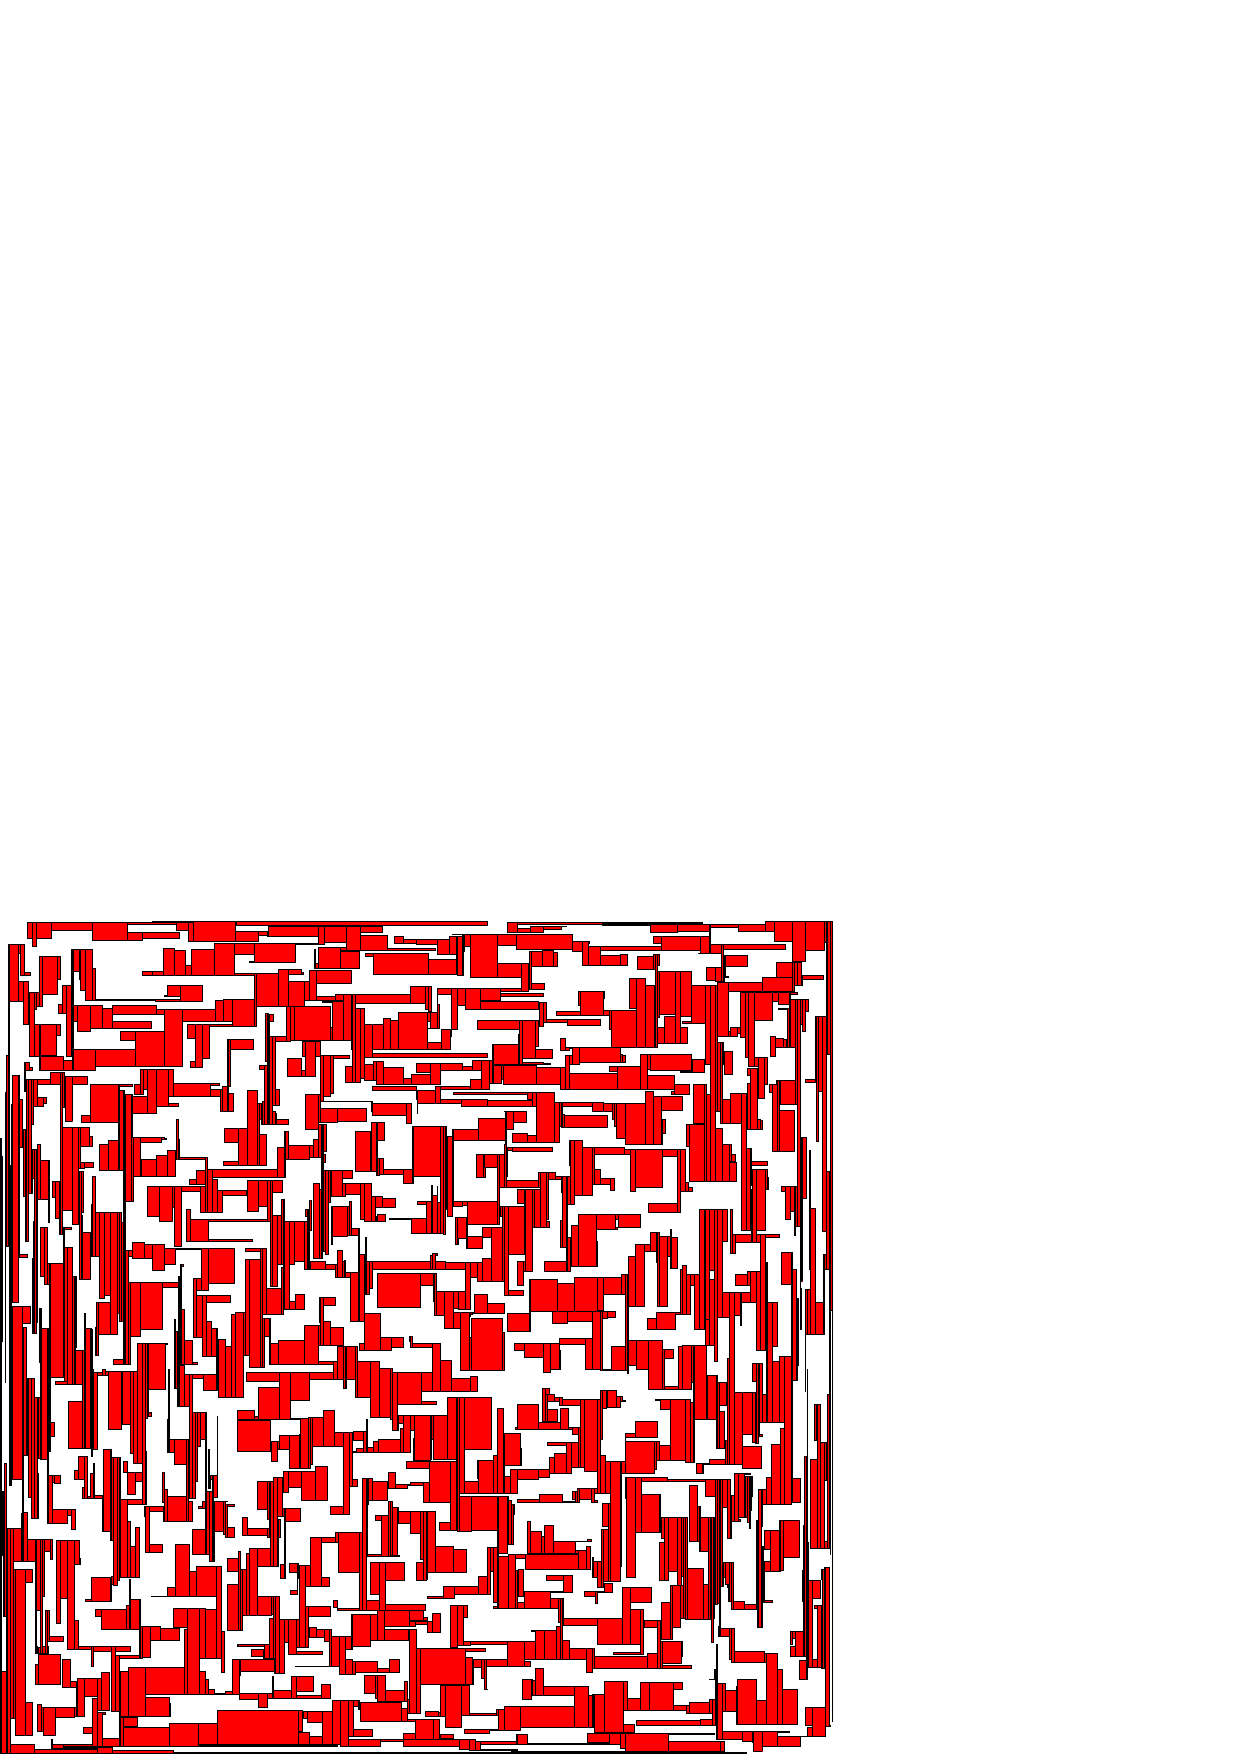
\includegraphics[width=1.0\textwidth]{polygon_cutting}}\\
  \caption{Polygon cutting.}\label{fig:polygon_cutting}
\end{figure}


Figure~\ref{fig:critical_area} shows an application of testing critical area
by polygon shrinking technique.

\begin{figure}[ht]
  \centering
  \scalebox{0.35}{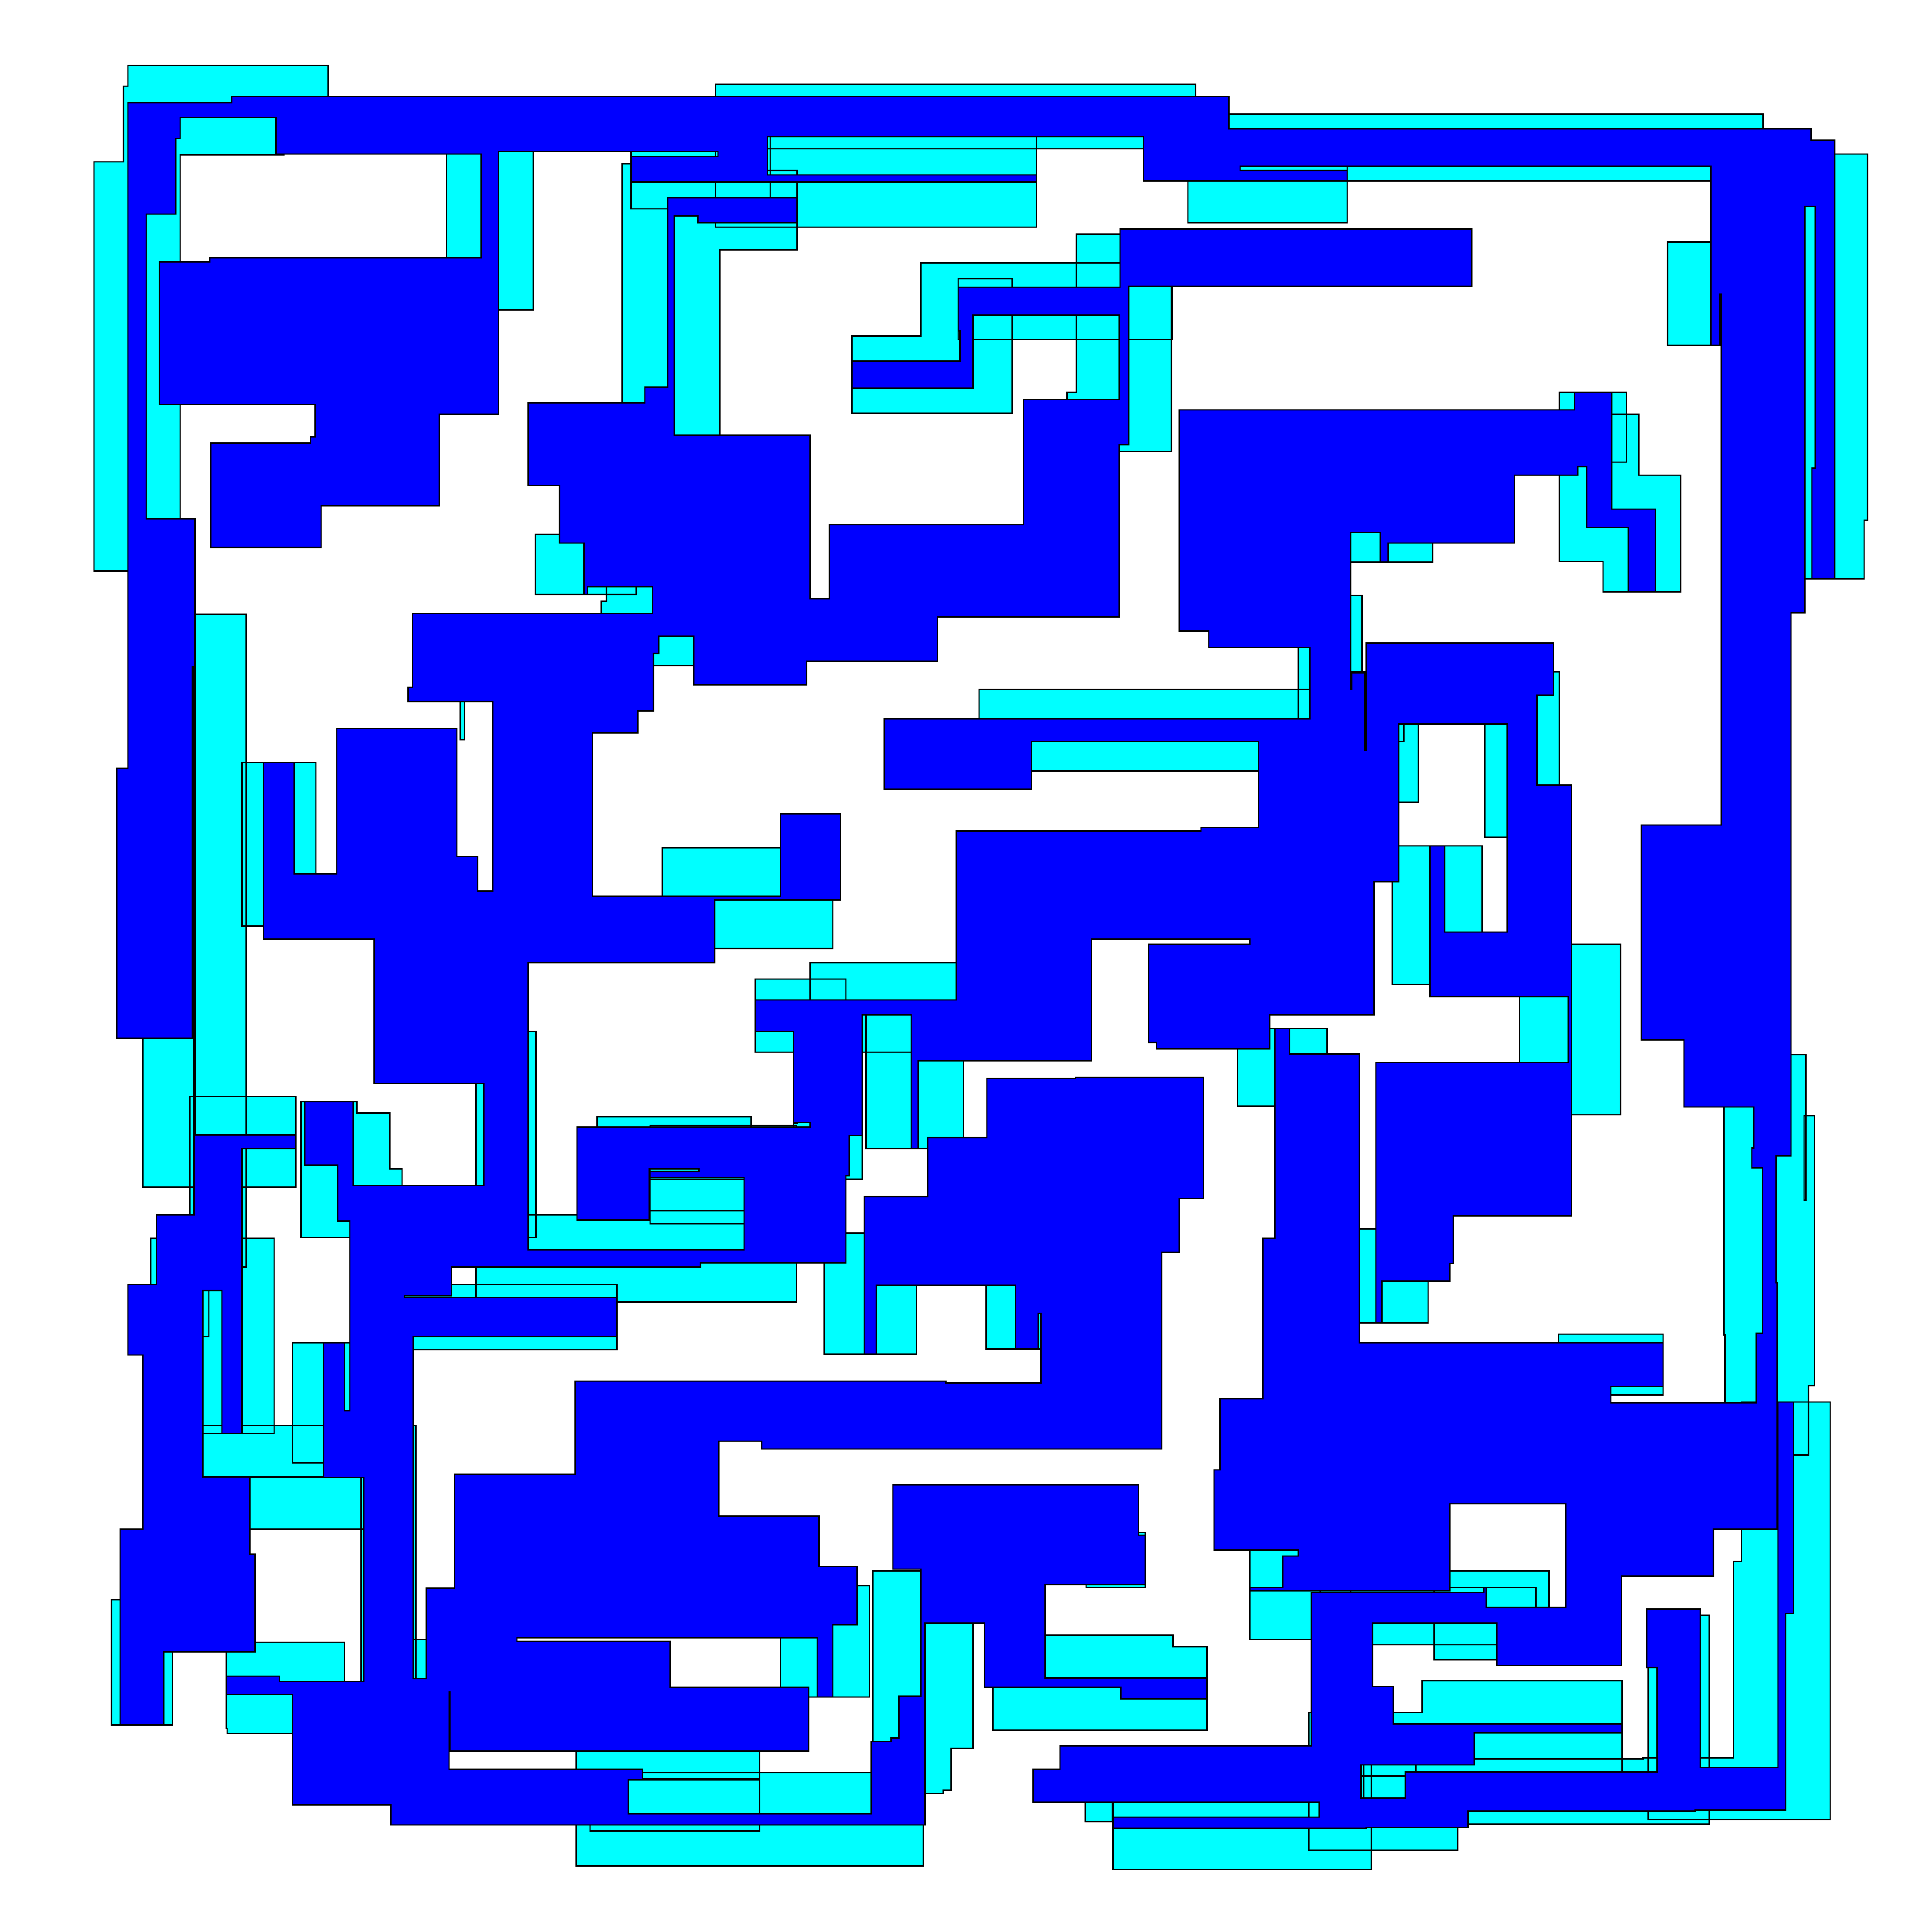
\includegraphics[width=1.0\textwidth]{critical_area}}\\
  \caption{Critical area.}\label{fig:critical_area}
\end{figure}


A typical layout feature is seldom as complicated as a random polygon. 
However, if an algorithm can handle this, it is likely that it can
handle all kind of layout features.  

\begin{figure}[ht]
  \centering
  \scalebox{0.35}{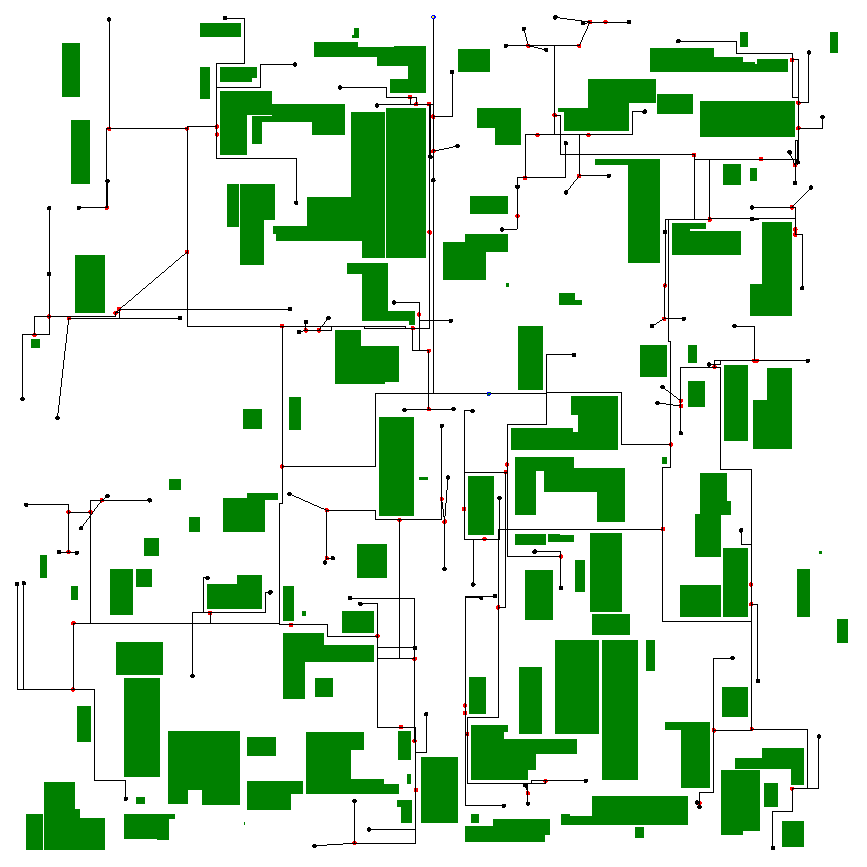
\includegraphics[width=1.0\textwidth]{Final_DmeObst_topology}}\\
  \caption{Testing clock tree synthesis with rectilinear obstacles}\label{fig:Final_DmeObst_topology}
\end{figure}

\section{Dynamic Priority Search Tree}
\label{sec:dyn-pst}
Priority search tree was first introduced in 80's. However, unlike
kd-tree~[], quad-tree~[], it has not been well noticed in EDA
community. One of the reasons may be that PST is only specialized in a
particular kind of range query, making it unsuitable for general
applications. Another reason is that the implementation of PST is not
trivial, especially one that requires dynamic balancing. 

\subsection{What is Priority Search Tree?}
Given a set of 2-dimensional point $(x,y)$.
Priority search tree is a data structure that organizes the data in a
binary search tree. It combines 1-D range tree
and a heap in one tree. It is particularly for the 2D range query in
the form of $([x_1:x_2], [-\infty:y]$. The dynamic version with
re-balancing uses for example red/black tree~[] or AVL tree~[] as the
basis of the 1d range-tree.
In our implementation, data are only stored in nodes. This is the key
different with other implementations.

A priority search tree has the following invariants
\begin{itemize}
\item
For any subtree rooted by $v$,
The $x$ values of lc($v$) is less than or equal to those of rc($v$) 
(binary search tree).
\item
The $y$ value of $v$ is smallest from its subtree (heap).
\item
If the underlying binary tree is a balanced binary tree
(e.g. Red-black tree), then it satifies the balance condition.
\end{itemize}

An example of a valid priority search tree is given in
Figure~\ref{fig:pst}. 

\begin{figure*}[ht]
  \centering
  \scalebox{0.8}{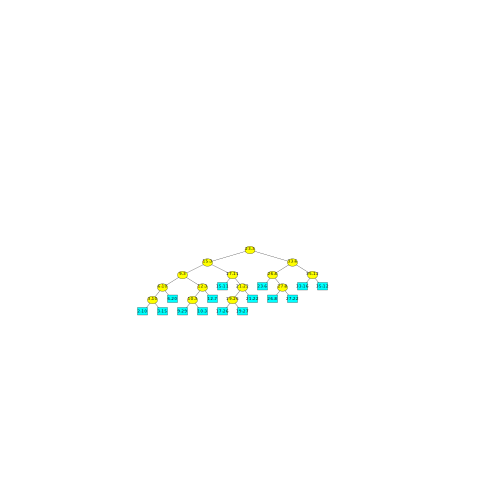
\includegraphics[width=1.0\textwidth]{pst}}\\
  \caption{Example of a valid priority search tree}\label{fig:pst}
\end{figure*}

\subsubsection{Insertion}


\begin{algorithm}[ht]
\caption{Insertion algorithm}
\label{alg:pst_insert}
    \begin{algorithmic}[1]
     \REQUIRE a PST tree $T$ and a point $(v,w)$
     \STATE Find a leaf node to be inserted according to the $v$ value.
    \end{algorithmic}
\end{algorithm}

\begin{figure*}[ht]
  \centering
  \scalebox{0.8}{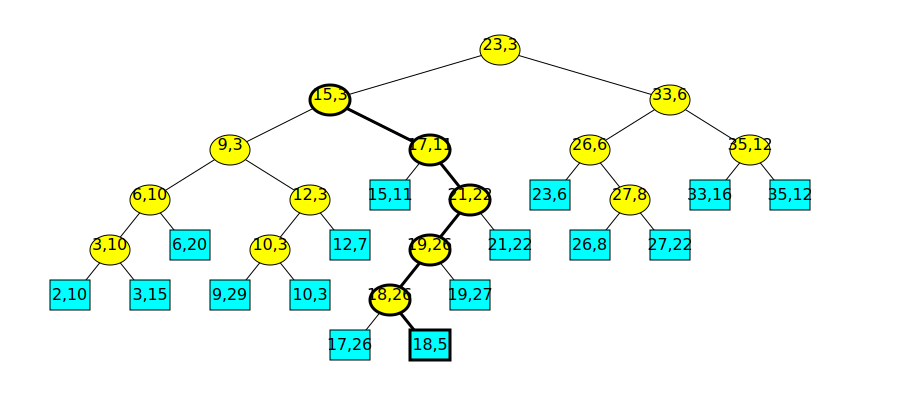
\includegraphics[width=1.0\textwidth]{pst_just_insert}}\\
  \caption{Insertion before tournament}\label{fig:pst_just_insert}
\end{figure*}

\begin{figure*}[ht]
  \centering
  \scalebox{0.8}{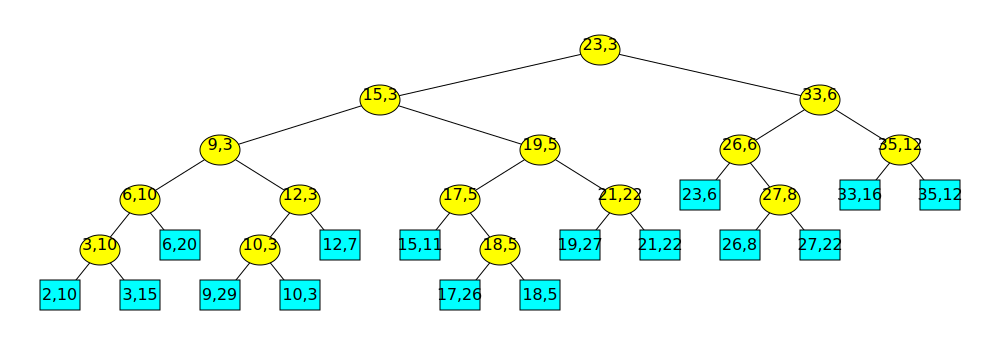
\includegraphics[width=1.0\textwidth]{pst_insert}}\\
  \caption{Insertion after re-balancing}\label{fig:pst_insert}
\end{figure*}

\subsubsection{Deletion}




\subsection{Applications of PST}
In~[], a list of applications are described. The main applications are
for interval set. With plane sweeping, dynamic PST can used for
finding all overlapping of a set of axis-parallel rectangles. For
example, in global placement. In~[], VLSI layout compaction use
radix-PST. It can be used for constructing conflict graphs in many
applications such as phase-shift masking (PSM).

\subsection{Range tree}

\subsection{Heap}

\subsection{}


\section{Experimental Results}
\label{sec:experiment}
Question 2: How many 2-opt moves need? $O(N^3)$? $O(N)$?

\begin{figure}[ht]
  \centering
  \scalebox{0.35}{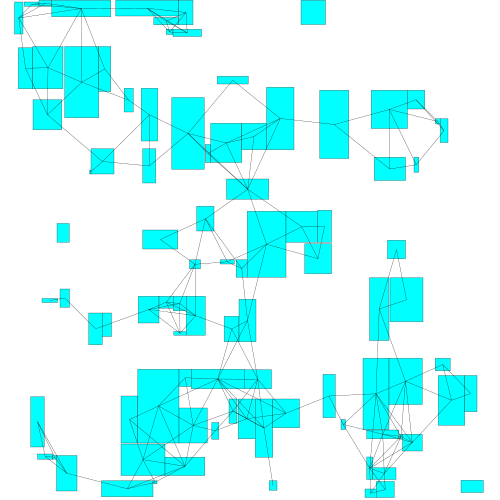
\includegraphics[width=1.0\textwidth]{conflict}}\\
  \caption{Conflict graph.}\label{fig:conflict}
\end{figure}


\section{Conclusions}
\label{sec:conclusions}

\bibliographystyle{unsrt}
\bibliography{random_pd}

\end{document}
